\section{Wahl der IMU} \label{imuWahl}
Das primäre Ziel für die IMU war die Möglichkeit die Heading möglichst genau zu
bestimmen. Im Vordergrund stand dabei eine hochwertige 6-Achsen-Fusion aus
Gyroskop und Accelerometer. Es sollte aber auch die Möglichkeit einer
9-Achsen-Fusion bestehen. Da aber nicht nicht Sicherstellbar im Anwendungsfall
von Smart Drive X4 die Nutzung von einem Magnetometer möglich sein könnte,
wurde besonders auf eine Solide 6 Achsen Fusion wert gelegt. Grund hierfür ist,
dass im Fahrzeug durch den Einsatz von Motoren, Stromleitungen sowie
ferromagnetischen Komponenten, dass die Messwerte des Magnetometer liefern kann
(vgl. Hardiron- und Softiron-Effekte im vorangegangenen Kapitel).
Verwertbare Messwerte liefert (vgl. Hard- und Softiron-Effekte im
vorangegangenen Kapitel).\\

\begin{minipage}[c]{0.55\textwidth}
\subsection{Gewählte IMU: LSM6DSV16X}
Die Wahl fiel auf die \textit{LSM6DSV16X} von STMicroelectronics. Sie ist eine
6 Achsen IMU und zeichnet sich besonders über ihre Low-Noice-Charakteristik aus,
wie auch den internen Motion-Processor (SFLP-Block). Diese Sensor Fusion Low
Power Einheit (SFLP) liefert unter anderem einen Game Rotation Vektor in
Quaternion Format und Gyro-Bias-Calibration. Alle Sensordaten und Fusiondaten des SFLP-Blocks können in
den internen FIFO. Dabei wird alles in Batches zusammengefasst und kann mit
einem Zeitstempel versehen werden.\\
Weiters verfügt der \textit{LSM6DSV16X} über eine Sensor-Hub-Funktionalität. 
Dabei agiert die IMU als I2C-Master und kann externe Sensoren auslesen. 
Diese Funktion wurde dafür genutzt werden ein externes Magnetometer an zu schließen,
die Messwerte über im FIFO zu speichern und diesen aus zu lesen.
Dies ist hilfreich weil alle Sensordaten an einem Zentralen Punkt ausgelesen werden konnten.
\end{minipage}
\hfill
\begin{minipage}[c]{0.4\textwidth}
    \centering
    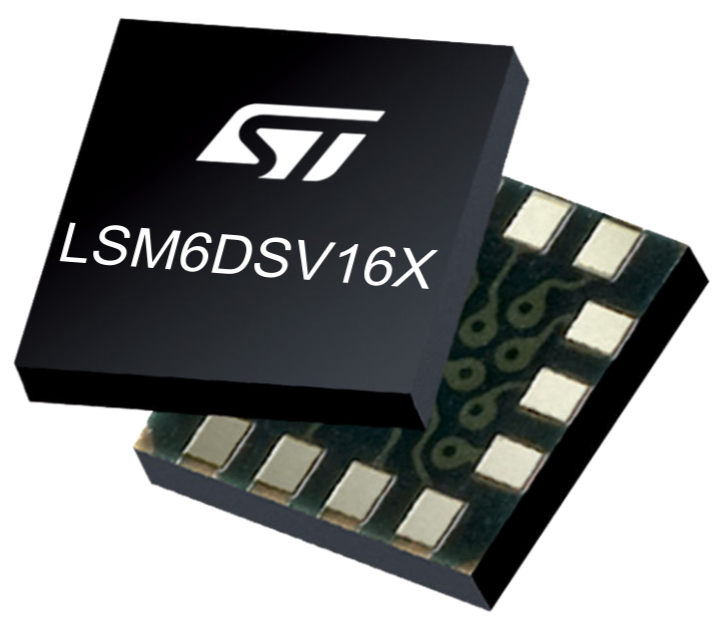
\includegraphics[width=\linewidth]{Bilder-Grafiken/Matthias/IMU/LSM6DSV16X_Package_Image.png}
    \captionof{figure}{LSM6DSV16X von STMicroelectronics, 6-Achsen IMU \cite{st_lsm6dsv16x}}
\end{minipage}

\subsection{Betrachtete Alternativen}
Als Alternativen wurden die \textit{ICM-42688-P} von TDK InvenSense \cite{tdk_icm42688p}
sowie die \textit{BNO086} von CEVA \cite{ceva_bno08x} evaluiert.
Die \textit{ICM-42688-P} ist eine 6 Achsen IMU mit ähnliche Low-Noice-Charakteristik
und Preis wie die \textit{LSM6DSV16X}, aber keinen internen Motion Processor und
Sensor-Hub. Die \textit{BNO086} ist eine 9 Achsen IMU mit integriertem 
32bit ARM Cortex-M0+ Core für Sensorfusion und Calibration.
Damit ist sie deutlich komplexer und auch
teurer. Noch dazu ist der interne Processor eine Black Box. \\
Es wurde die \textit{LSM6DSV16X} gewählt weil sie im Vergleich zu der
\textit{BNO086} mehr Flexibilität bietet, jedoch mehr features wie die
\textit{ICM-42688-P} bietet.

\section{Wahl des Magnetometers}
Für die angestrebte 9-Achsen-Fusion ist ein zusätzliches Magnetometer
erforderlich. Wie schon erwähnt, kann die \textit{LSM6DSV16X} als Sensor-Hub
agieren. STMicroelectronics selbst bietet ein Example an, bei das
\textit{LIS2MDL} Magnetometer über den Sensor-Hub ausgelesen wird. Für Smart
Drive X4 wurde die \textit{LIS2MDL} gewählt, da die Implementierung durch die
Beispiele schon existierte und dies somit keine Eigenimplementation erfolgen
muss. 
